\documentclass[main.tex]{subfiles}
% CONCEPTS
\begin{document}
  % Data Structure
  % Trace by Trace Anaysis
    % Points of Interest
    % Polynomal
    % Exponential
  % Limitations
    % Trigonometric
      % Use FFT
    % Nested Functions
    % Noise vs Precision
      % Typical Trade Off
  The derivative analysis builds mainly on a matrix, beginning with the actual data values (derivative 0), followed by the derivatives along the "depth" of the matrix. This is demonstrated in \cref{tbl:mtrx:simple} with a parabola. The depth that the matrix reaches before becoming zero in a particular column defines that data point's derivative depth or \textit{derivDepth}.
  \subfile{tables/simpleMatrix}
  
  \section{Derivative Characteristics}
    
    Due to its simplicity, most classification is best performed while making use of the polynomial classification.
    
    \begin{figure}[h]
      \begin{subfigure}{0.48\linewidth}
        \centering
        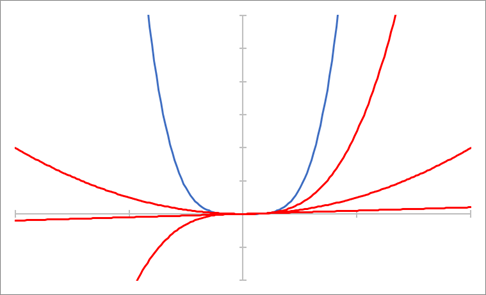
\includegraphics[width=0.9\linewidth]{figures/derivPoly}
        \caption{Polynomials}
        \label{fig:deriv:poly}
      \end{subfigure}
      \begin{subfigure}{0.48\linewidth}
        \centering
        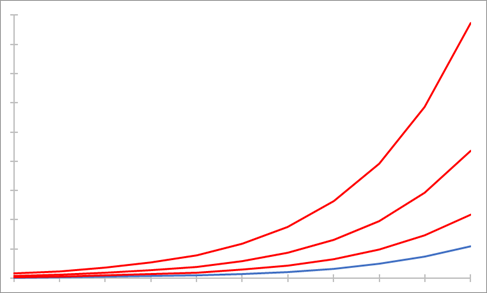
\includegraphics[width=0.9\linewidth]{figures/derivExp}
        \caption{Exponential}
        \label{fig:deriv:exp}
      \end{subfigure}
      \caption{Derivative patterns of (\subref{fig:deriv:poly}) polynomial and \subref{fig:deriv:exp}) exponential functions. (\subref{fig:deriv:poly}) shows a fourth order polynomial in blue ($x^4$) and its derivatives in red, a third ($x^3$), second ($x^2$) and first ($x$) order polynomial, which a "zeroth" order polynomial ($x^0$ or simply $1$) follows, but is too small do display. No further derivatives would follow. (\subref{fig:deriv:exp}) shows an exponential of the form $e^{a x}$ in blue, with $a>1$ and hence its derivatives growing larger with the level of derivative, by $a$, $a^2$ and $a^3$ respectively. (\subref{fig:deriv:exp}) will never reach a zero derivative.}
      \label{fig:deriv}
    \end{figure}
    
    \subsection{Polynomials}
    
      By far the simplest functions to classify are \textbf{polynomials}. Any polynomial of degree $N$ will have exactly $N$ non-zero derivatives (also see \cref{fig:deriv:poly}), and so it is only necessary to count the number of times that the derivative is not zero i.e. the \textit{derivDepth}. If it never becomes zero then the data is not polynomial, or we have not taken enough derivatives.
    
    \subsection{Nested Functions}
      
      As stated in \cref{sec:back:combFunc}, there are limitations to the amount of analysis that can be performed on combined functions. However, the most common functions can be easily covered, by applying their inverse after classifying a segment as not-polynomial. First the Natural Logarithm is applied to the data segment in question, which is then analysed again. If it is classified as a polynomial at this stage the original data segment can be marked as exponential. While further analysis is not yet implemented, similar processes will allow classification of rational and root functions, as well as logarithmic functions.
      \\\\
      Note, however, in \cref{fig:deriv:exp}, how towards the left side the exponentials approximate to zero. All exponentials have such an asymptote, where they approximate a constant of zero to infinite precision. There is no mathematical means to tell this segment apart from a true constant, without the additional information from other data segments or infinite precision that no sensor can provide. At this time this classification is considered accurate, but it can be adjusted for in the next analysis step, when information from more than one data point at a time is used to continue analysis. Similar segments exist in logarithmic and rational functions.
      
    \subsection{Points of Interest}
      
      \subfile{tables/poiMatrix}
      
  \section{Precision}
  

  
  
\end{document}